\documentclass[12pt,letterpaper]{article}
\usepackage{graphicx,textcomp}
\usepackage{natbib}
\usepackage{setspace}
\usepackage{fullpage}
\usepackage{color}
\usepackage[reqno]{amsmath}
\usepackage{amsthm}
\usepackage{fancyvrb}
\usepackage{amssymb,enumerate}
\usepackage[all]{xy}
\usepackage{endnotes}
\usepackage{lscape}
\newtheorem{com}{Comment}
\usepackage{float}
\usepackage{hyperref}
\newtheorem{lem} {Lemma}
\newtheorem{prop}{Proposition}
\newtheorem{thm}{Theorem}
\newtheorem{defn}{Definition}
\newtheorem{cor}{Corollary}
\newtheorem{obs}{Observation}
\usepackage[compact]{titlesec}
\usepackage{dcolumn}
\usepackage{tikz}
\usetikzlibrary{arrows}
\usepackage{multirow}
\usepackage{xcolor}
\newcolumntype{.}{D{.}{.}{-1}}
\newcolumntype{d}[1]{D{.}{.}{#1}}
\definecolor{light-gray}{gray}{0.65}
\usepackage{url}
\usepackage{listings}
\usepackage{color}

\definecolor{codegreen}{rgb}{0,0.6,0}
\definecolor{codegray}{rgb}{0.5,0.5,0.5}
\definecolor{codepurple}{rgb}{0.58,0,0.82}
\definecolor{backcolour}{rgb}{0.95,0.95,0.92}

\lstdefinestyle{mystyle}{
	backgroundcolor=\color{backcolour},   
	commentstyle=\color{codegreen},
	keywordstyle=\color{magenta},
	numberstyle=\tiny\color{codegray},
	stringstyle=\color{codepurple},
	basicstyle=\footnotesize,
	breakatwhitespace=false,         
	breaklines=true,                 
	captionpos=b,                    
	keepspaces=true,                 
	numbers=left,                    
	numbersep=5pt,                  
	showspaces=false,                
	showstringspaces=false,
	showtabs=false,                  
	tabsize=2
}
\lstset{style=mystyle}
\newcommand{\Sref}[1]{Section~\ref{#1}}
\newtheorem{hyp}{Hypothesis}

\title{Problem Set 3}
\date{Due: March 25, 2026}
\author{Applied Stats II}


\begin{document}
	\maketitle
	\section*{Instructions}
	\begin{itemize}
	\item Please show your work! You may lose points by simply writing in the answer. If the problem requires you to execute commands in \texttt{R}, please include the code you used to get your answers. Please also include the \texttt{.R} file that contains your code. If you are not sure if work needs to be shown for a particular problem, please ask.
\item Your homework should be submitted electronically on GitHub in \texttt{.pdf} form.
\item This problem set is due before 23:59 on Wednesday March 25, 2026. No late assignments will be accepted.
	\end{itemize}

	\vspace{.25cm}
\section*{Question 1}
\vspace{.25cm}
\noindent We are interested in how governments' management of public resources impacts economic prosperity. Our data come from \href{https://www.researchgate.net/profile/Adam_Przeworski/publication/240357392_Classifying_Political_Regimes/links/0deec532194849aefa000000/Classifying-Political-Regimes.pdf}{Alvarez, Cheibub, Limongi, and Przeworski (1996)} and is labelled \texttt{gdpChange.csv} on GitHub. The dataset covers 135 countries observed between 1950 or the year of independence or the first year forwhich data on economic growth are available ("entry year"), and 1990 or the last year for which data on economic growth are available ("exit year"). The unit of analysis is a particular country during a particular year, for a total $>$ 3,500 observations. 

\begin{itemize}
	\item
	Response variable: 
	\begin{itemize}
		\item \texttt{GDPWdiff}: Difference in GDP between year $t$ and $t-1$. Possible categories include: "positive", "negative", or "no change"
	\end{itemize}
	\item
	Explanatory variables: 
	\begin{itemize}
		\item
		\texttt{REG}: 1=Democracy; 0=Non-Democracy
		\item
		\texttt{OIL}: 1=if the average ratio of fuel exports to total exports in 1984-86 exceeded 50\%; 0= otherwise
	\end{itemize}
	
\end{itemize}
\newpage
\noindent Please answer the following questions:

\begin{enumerate}
	\item Construct and interpret an unordered multinomial logit with \texttt{GDPWdiff} as the output and "no change" as the reference category, including the estimated cutoff points and coefficients.\\
	
	First, it seemed unusual to me to have three categories ("negative change", "no change" and "positive change") with such extreme variation in their ranges. Further, with "no change" category set only to countries that saw exactly 0 change in their GDP, I felt interpretability would be weak. As such, I set my "no change" category for any GDP changes lying between -25 and +25 (this is reasonable to account for noise, minor changes over time, and helps give the "no change" category reasonable comparative value against the other two categories).  Visualizing the data helped me ensure my range (-25 - +25) was reasonable as well.\\
	
		\lstinputlisting[language=R, firstline=37, lastline=49]{PS03_SVU.R}
	
	\begin{figure}[h!]
		\caption{Majority of the GDP Change Distribution}\label{fig1}
		\centering
		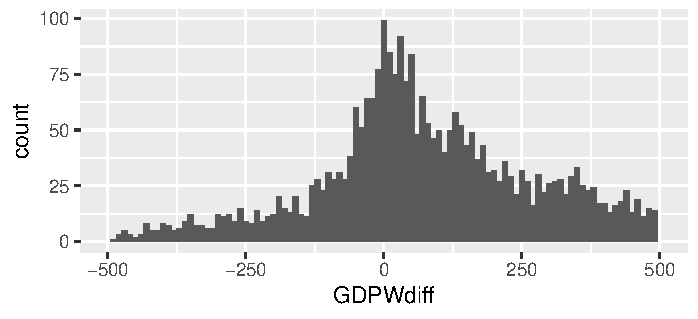
\includegraphics[width=.8\textwidth]{basic_viz.pdf}
	\end{figure}
	
	
	I fit the model to other cutoff ranges as well to check for robustness, and the overall trend is the same: REG (regime type) has, on average, a consistently stronger impact on GDP change category than does the OIL (oil as export majority) variable. Here's the code for setting up the model:
	
		\lstinputlisting[language=R, firstline=51, lastline=65]{PS03_SVU.R}
	
	\begin{table}[!htbp] \centering 
		\caption{Unordered Multinomial Logistic Regression} 
		\label{} 
		\begin{tabular}{@{\extracolsep{5pt}}lcc} 
			\\[-1.8ex]\hline 
			\hline \\[-1.8ex] 
			& \multicolumn{2}{c}{\textit{Dependent variable:}} \\ 
			\cline{2-3} 
			\\[-1.8ex] & negative change & positive change \\ 
			\\[-1.8ex] & (1) & (2)\\ 
			\hline \\[-1.8ex] 
			OIL & 0.846$^{***}$ & 0.575$^{***}$ \\ 
			& (0.221) & (0.210) \\ 
			& & \\ 
			REG & 1.014$^{***}$ & 1.355$^{***}$ \\ 
			& (0.146) & (0.135) \\ 
			& & \\ 
			Constant & 0.455$^{***}$ & 1.306$^{***}$ \\ 
			& (0.072) & (0.064) \\ 
			& & \\ 
			\hline \\[-1.8ex] 
			Akaike Inf. Crit. & 6,357.149 & 6,357.149 \\ 
			\hline 
			\hline \\[-1.8ex] 
			\textit{Note:}  & \multicolumn{2}{r}{$^{*}$p$<$0.1; $^{**}$p$<$0.05; $^{***}$p$<$0.01} \\ 
		\end{tabular} 
	\end{table}
	
	The coefficients tell us that these variables have statistical significance in both positive and negative change in GDP for the countries. Each indicates a difference in the log-odds of being in the category for which they're calculated ("negative change" or "positive change") as compared to the reference category, "no change." For example, a country having more than 50 percent of its exports dedicated to oil will (on average, holding all else constant) have 0.575 units higher log-odds of being in the "positive change" than being in the "no-change" GDP category. Exponentiating this coefficient gives it more meaning, as $e^{0.575} \approx 1.777$ indicates that oil-dependent economies will have 77 percent higher odds of being in the "positive change" category as opposed to the "no change" category.\\
	
	
	Below I estimate z- and p-values to help validate these results:\\
	
	\begin{table}[ht]
		\centering
		\caption{Z-Values for Unordered Logit Coefficients}
		\begin{tabular}{rrrr}
			\hline
			& (Intercept) & OIL & REG \\ 
			\hline
			negative change & 6.31$^{***}$ & 3.83$^{***}$ & 6.93$^{***}$ \\ 
			positive change & 20.47$^{***}$ & 2.74$^{**}$ & 10.01$^{***}$ \\ 
			\hline \\[-1.8ex]
			\textit{Note:}  & \multicolumn{2}{r}{$^{*}$p$<$0.1; $^{**}$p$<$0.05; $^{***}$p$<$0.01} \\ 
		\end{tabular}
	\end{table}
	
			\lstinputlisting[language=R, firstline=68, lastline=71]{PS03_SVU.R}
	
	\item Construct and interpret an ordered multinomial logit with \texttt{GDPWdiff} as the outcome variable, including the estimated cutoff points and coefficients.
	
	Theoretically speaking, an ordered multinomial logit makes sense as there is an interpretable order between categories of change for GDPs. Re-leveling the factor of the output variable \texttt{GDPWdiff} and running the \texttt{polr()} function returns the following regression output:\\
	
				\lstinputlisting[language=R, firstline=75, lastline=82]{PS03_SVU.R}
				
				
	\begin{table}[!htbp] \centering 
		\caption{Ordered Multinomial Logistic Regression} 
		\label{} 
		\begin{tabular}{@{\extracolsep{5pt}}lc} 
			\\[-1.8ex]\hline 
			\hline \\[-1.8ex] 
			& \multicolumn{1}{c}{\textit{Dependent variable:}} \\ 
			\cline{2-2} 
			\\[-1.8ex] & GDP\_ordered \\ 
			\hline \\[-1.8ex] 
			OIL & $-$0.148 \\ 
			& (0.112) \\ 
			& \\ 
			REG & 0.502$^{***}$ \\ 
			& (0.072) \\ 
			& \\ 
			\hline \\[-1.8ex] 
			AIC & 6438.58 \\ 
			Observations & 3,721 \\ 
			\hline 
			\hline \\[-1.8ex] 
			\textit{Note:}  & \multicolumn{1}{r}{$^{*}$p$<$0.1; $^{**}$p$<$0.05; $^{***}$p$<$0.01} \\ 
		\end{tabular} 
	\end{table} 
	
	The \texttt{OIL} coefficient indicates that, holding all else constant, countries with >50 percent of their exports in oil have a log-odds that is (on average) 0.148 units lower (than others) of being in a higher GDP growth category. Exponentiating the coefficient, $e^{-0.148} \approx 0.862$, implies that oil-dependent countries have approximately 13.8 percent lower odds of being in a higher GDP growth category compared to non-oil-dependent countries. However, this effect is not statistically significant.\\
	
	In contrast, the \texttt{REG} coefficient does hold statistical significance and evidences that, on average and with all else held constant, democracies have 0.502 higher log-odds of being in a higher GDP growth category than other regimes. In exponentiated terms ($e^{0.502} \approx 1.652$), democracies have 65.2 percent higher odds of being in a higher GDP growth category compared to non-democracies.\\
	
	See summary tables 4 and 5 which display the coefficients once more, with t- and p-values, cutoff values for categorizing the inputs by the log-odds output (-0.96 for negative - no change, -0.42 for no - positive change), and odds ratios with confidence intervals for each coefficient respectively.\\
	
				\lstinputlisting[language=R, firstline=86, lastline=92]{PS03_SVU.R}
	
	\begin{table}[ht]
		\caption{Coefficients and Cutoff Values For Ordered Logit} 
		\centering
		\begin{tabular}{rrrrr}
			\hline
			& Value & Std. Error & t value & p value \\ 
			\hline
			OIL & -0.15 & 0.11 & -1.33 & 0.18 \\ 
			REG & 0.50 & 0.07 & 7.02 & 0.00 \\ 
			\hline
			negative change$|$no change & -0.96 & 0.05 & -20.28 & 0.00 \\ 
			no change$|$positive change & -0.42 & 0.04 & -9.47 & 0.00 \\ 
			\hline
		\end{tabular}
	\end{table}
	
	\newpage
	
	\begin{table}[ht]
		\centering
		\caption{Odds Ratios and Confidence Intervals for Ordered Logit Variables}
		\begin{tabular}{rrrr}
			\hline
			& OR & 2.5 \% & 97.5 \% \\ 
			\hline
			OIL & 0.86 & -0.37 & 0.07 \\ 
			REG & 1.65 & 0.36 & 0.64 \\ 
			\hline
		\end{tabular}
	\end{table}
	
	
\end{enumerate}

\newpage

\section*{Question 2} 
\vspace{.25cm}

\noindent Consider the data set \texttt{MexicoMuniData.csv}, which includes municipal-level information from Mexico. The outcome of interest is the number of times the winning PAN presidential candidate in 2006 (\texttt{PAN.visits.06}) visited a district leading up to the 2009 federal elections, which is a count. Our main predictor of interest is whether the district was highly contested, or whether it was not (the PAN or their opponents have electoral security) in the previous federal elections during 2000 (\texttt{competitive.district}), which is binary (1=close/swing district, 0="safe seat"). We also include \texttt{marginality.06} (a measure of poverty) and \texttt{PAN.governor.06} (a dummy for whether the state has a PAN-affiliated governor) as additional control variables. 

\begin{enumerate}
	\item [(a)]
	Run a Poisson regression because the outcome is a count variable. Is there evidence that PAN presidential candidates visit swing districts more? Provide a test statistic and p-value.\\
	
	First of all, upon initial visualizations, it's noticeable that there is a single outlier point in this dataset (see Figure ~\ref{fig2}). I ran the following outputs with and without it, but the results don't vary terribly much. Either way, as there was no instruction to remove outliers, I've kept the outlier in, but include a table of regression coefficients for the model with the outlier excluded at the end (see Table ~\ref{tab_outlier}).
	
				\lstinputlisting[language=R, firstline=126, lastline=127]{PS03_SVU.R}
	
	\begin{figure}[h!]
		\caption{Outlier in the Data - PAN Pres Candidate Visits to Competitive Districts}\label{fig2}
		\centering
		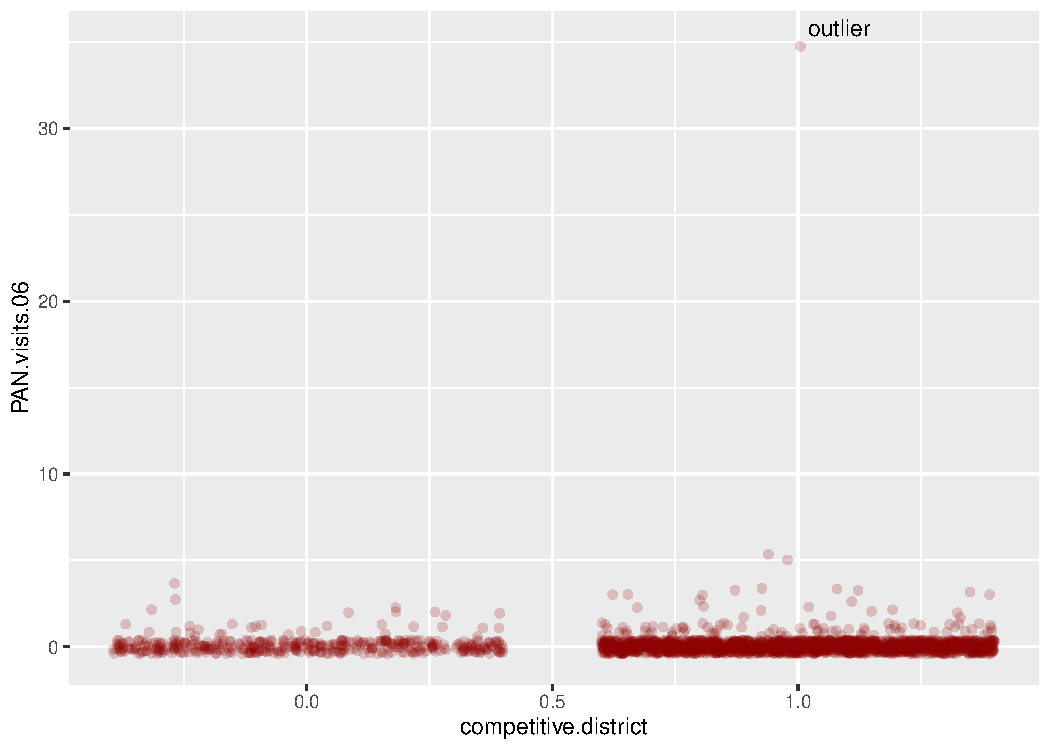
\includegraphics[width=.75\textwidth]{outlier.pdf}
	\end{figure}
	
			\lstinputlisting[language=R, firstline=132, lastline=138]{PS03_SVU.R}
			\newpage
			
			For creating our model and assessing it:
			
			\lstinputlisting[language=R, firstline=147, lastline=153]{PS03_SVU.R}
			\newpage
			\begin{table}[!htbp] \centering 
				\caption{Poisson Regression} 
				\label{} 
				\begin{tabular}{@{\extracolsep{5pt}}lc} 
					\\[-1.8ex]\hline 
					\hline \\[-1.8ex] 
					& \multicolumn{1}{c}{\textit{Dependent variable:}} \\ 
					\cline{2-2} 
					\\[-1.8ex] & PAN.visits.06 \\ 
					\hline \\[-1.8ex] 
					competitive.district & $-$0.081 \\ 
					& (0.171) \\ 
					& \\ 
					marginality.06 & $-$2.080$^{***}$ \\ 
					& (0.117) \\ 
					& \\ 
					PAN.governor.06 & $-$0.312$^{*}$ \\ 
					& (0.167) \\ 
					& \\ 
					Constant & $-$3.810$^{***}$ \\ 
					& (0.222) \\ 
					& \\ 
					\hline \\[-1.8ex] 
					Observations & 2,407 \\ 
					Log Likelihood & $-$645.606 \\ 
					Akaike Inf. Crit. & 1,299.213 \\ 
					\hline 
					\hline \\[-1.8ex] 
					\textit{Note:}  & \multicolumn{1}{r}{$^{*}$p$<$0.1; $^{**}$p$<$0.05; $^{***}$p$<$0.01} \\ 
				\end{tabular} 
			\end{table} 
		
			
			As we are working with a Poisson regression, the coefficients indicate the variables' impact on the log-count of the outcome variable. For the research question at hand (do successful PAN presidential candidates visit swing districts more frequently than the rest?), the coefficients indicate a slight negative but \textbf{non-significant} relationship. According to our model, holding all else constant, for competitive ("swing") districts, a $e^{-0.081} = 0.922$ multiplicative decrease (8.8 percent fewer) in visits is expected on average. The z-value for this coefficient is 1.763, with a  p-value of 0.78, indicating non-significance.\\
			
Dispersion testing indicated no evidence of overdispersion, but I did go ahead and run a zero-inflation model and negative binomial model, as I thought they might show some evidence of better fit, and indeed they improve on the AIC scoring (see Table 6), but I'll continue my analysis using the basic Poisson model.\\

		\lstinputlisting[language=R, firstline=155, lastline=158]{PS03_SVU.R}
		\lstinputlisting[language=R, firstline=172, lastline=173]{PS03_SVU.R}

	\begin{table}[ht]
		\centering
		\label{tab6}
		\caption{AICs for Different Model Fits} 
		\begin{tabular}{rrr}
			\hline
			Model Name & df & AIC \\ 
			\hline
			Poisson & 4.00 & 1299.21 \\ 
			Zero-Inflation & 8.00 & 1216.77 \\ 
			Negative Binomial & 5.00 & 1081.91 \\ 
			\hline
		\end{tabular}
	\end{table}


	\item [(b)]
	Interpret the \texttt{marginality.06} and \texttt{PAN.governor.06} coefficients.\\
	
	 	 \texttt{marginality.06}: \textbf{-2.08} -- A one unit increase in the marginality index results in a 2.08 decrease in the log of predicted district visits by the winning PAN predidential candidate, on average and holding all else constant. In clearer terms, a one unit increase in the marginality index results in a $e^{-2.08} = 0.125$ multiplicative decrease in expected visits on average (87.5 percent fewer visits per increase in marginality index, on average). \\
	
		\texttt{PAN.governor.06}: \textbf{-0.312} -- Districts with PAN-affiliated governors have a 0.312-point smaller log-count of predicted district visits by the winning PAN presidential candidate, on average, than districts without PAN-affiliated governors (holding all else constant). Again, in other terms, districts with PAN-affiliated governors receive $e^{-0.312} = 0.732$ times as many (26.8 percent fewer) visits on average as districts without PAN-affiliated governors.
	
	
	\item [(c)]
	Provide the estimated mean number of visits from the winning PAN presidential candidate for a hypothetical district that was competitive (\texttt{competitive.district}=1), had an average poverty level (\texttt{marginality.06} = 0), and a PAN governor (\texttt{PAN.governor.06}=1).\\
	
		By hand or using \texttt{predict} in \texttt{R}, we find from the basic Poisson model that the mean visits of from the winning PAN presidential candidate to the hypothetical district is 0.015.\\
	
	By hand:\\
	
		\lstinputlisting[language=R, firstline=187, lastline=189]{PS03_SVU.R}
	
	Using \texttt{predict}:\\
	
		\lstinputlisting[language=R, firstline=178, lastline=185]{PS03_SVU.R}


Without the outlier, the Poisson's predicted average visits to the hypothetical district goes up to 0.0163. Though the AIC is 1051, the dispersion test output suggests we are overdispersed. See Poisson model coefficients with the outlier excluded below:\\


	\begin{table}[!htbp] \centering 
		\caption{Poisson Regression (w/out Outlier)} 
		\label{tab_outlier} 
		\begin{tabular}{@{\extracolsep{5pt}}lc} 
			\\[-1.8ex]\hline 
			\hline \\[-1.8ex] 
			& \multicolumn{1}{c}{\textit{Dependent variable:}} \\ 
			\cline{2-2} 
			\\[-1.8ex] & PAN.visits.06 \\ 
			\hline \\[-1.8ex] 
			competitive.district & $-$0.261 \\ 
			& (0.176) \\ 
			& \\ 
			marginality.06 & $-$1.954$^{***}$ \\ 
			& (0.124) \\ 
			& \\ 
			PAN.governor.06 & $-$0.129 \\ 
			& (0.172) \\ 
			& \\ 
			Constant & $-$3.727$^{***}$ \\ 
			& (0.227) \\ 
			& \\ 
			\hline \\[-1.8ex] 
			Observations & 2,406 \\ 
			Log Likelihood & $-$521.651 \\ 
			Akaike Inf. Crit. & 1,051.301 \\ 
			\hline 
			\hline \\[-1.8ex] 
			\textit{Note:}  & \multicolumn{1}{r}{$^{*}$p$<$0.1; $^{**}$p$<$0.05; $^{***}$p$<$0.01} \\ 
		\end{tabular} 
	\end{table} 
	
\end{enumerate}

\end{document}
